\subsection{The Bin Packing Problem (bin\_pack\_func.py and bin\_pack\_instance.py)} \label{sbs:binpack}

The solution of the bin packing problem determines where, amongst $m$ ``bins'', to place $n$ ``items'' of various ``volumes'' in a way that (in this case study) minimises the wasted ``capacity'' of the bins. Each product $j=1, \ldots, n$ has a volume $v_j$ and each bin has capacity $C$. Extensions of this problem arise often in \ac{MILP} in problems including network design and rostering.

The \ac{MILP} formulation of the bin packing problem is straightforward. The decision variables are
\begin{align*}
x_{ij} &= \begin{cases} 1 & \text{if item $j$ is placed in bin $i$} \\
0 & \text{otherwise} \end{cases} \\
y_i &= \begin{cases} 1 & \text{if a facility is located at location $i$} \\
0 & \text{otherwise} \end{cases} \\
w_i &= \text{ ``wasted'' capacity at location $i$}
\end{align*}
and the formulation is
\[
\begin{array}{rr@{\ }ll}
       \min & \displaystyle \sum_{i=1}^m w_i \\
\text{s.t.} & \displaystyle \sum_{i=1}^m x_{ij}           & = 1, j = 1, \ldots, n      & \text{ (each product produced)} \\
            & \displaystyle \sum_{j=1}^n v_j x_{ij} + w_i & = C y_i, i = 1, \ldots, m  & \text{ (aggregate capacity at location $i$)} \\
            & \multicolumn{2}{l}{x_{ij} \leq y_i, i = 1, \ldots, m, j = 1, \ldots, n}  & \text{ (disaggregate capacity at location $i$)} \\[6pt]
            & \multicolumn{3}{l}{x_{ij} \in \{ 0, 1\}, w_i \geq 0, y_i \in \{0, 1\}, i = 1, \ldots, m, j = 1, \ldots, n}
\end{array}
\]

Note that the disaggregate capacity constraints are not necessary for defining the solution, but tighten the \ac{MILP} formulation (i.e., remove factional solutions from the solution space). Using PuLP we can easily define and solve this \ac{MILP} problem in Dippy. The formulation and solution functions from bin\_pack\_func.py are given below with a summary for each fragment.

\begin{enumerate}[leftmargin=0cm,itemindent=0.75cm,labelwidth=.5cm,labelsep=.25cm,labelindent=0cm,align=left]
\item Load PuLP and Dippy;
\lstinputlisting[firstnumber=12,linerange=12-30]{../../examples/Dippy/bpp/bin_pack_func.py}

\item Define \lstinline{BinPackProb}, a class that describes a bin packing problem;
\lstinputlisting[firstnumber=34,linerange=34-40]{../../examples/Dippy/bpp/bin_pack_func.py}

\item Define the \lstinline{formulate} function, with a bin packing problem object as input;
\begin{enumerate}[leftmargin=0cm,itemindent=0.75cm,labelwidth=.5cm,labelsep=.25cm,labelindent=0cm,align=left]
\item Create a \lstinline{DipProblem} (with some display options defined);
\lstinputlisting[firstnumber=42,linerange=42-47]{../../examples/Dippy/bpp/bin_pack_func.py}

\item Using the bin packing problem object's data (i.e., the data defined within \lstinline{bpp}), create the decision variables;
\lstinputlisting[firstnumber=49,linerange=49-54]{../../examples/Dippy/bpp/bin_pack_func.py}
\item and the objective function;
\lstinputlisting[firstnumber=56,linerange=56-56]{../../examples/Dippy/bpp/bin_pack_func.py}
\item and constraints;
\lstinputlisting[firstnumber=58,linerange=58-68]{../../examples/Dippy/bpp/bin_pack_func.py}

\vspace*{1cm} % \newpage destroys list spacing so pushing item down

\item Finally, the bin packing problem object and the decision variables are all ``embedded'' within the \lstinline{DipProblem} object, \lstinline{prob}, and this object is returned (note that the objective function and constraints could also be similarly embedded).
\lstinputlisting[firstnumber=82,linerange=82-89]{../../examples/Dippy/bpp/bin_pack_func.py}
\end{enumerate}

\item Define the \lstinline{solve} function that only requires a \lstinline{DipProblem} object, \lstinline{prob}, (note that no \lstinline{dippyOpts} are specified, so the Dippy defaults are used).
\lstinputlisting[firstnumber=123,linerange={123-124,132-132,143-148}]{../../examples/Dippy/bpp/bin_pack_func.py}

\end{enumerate}

To solve an instance of the bin packing problem, the data needs to be specified and then the problem formulated and solved as demonstrated in the file bin\_pack\_instance.py.
\lstinputlisting[firstnumber=3,linerange=3-22]{../../examples/Dippy/bpp/bin_pack_instance.py}

Solving this bin packing problem instance in Dippy gives the branch-and-bound tree shown in figure \ref{fig:bpp_tree1} (note that the integer solution found -- indicated in blue \lstinline{S: 5.0} -- bounds all other nodes in the tree) with the final solution packing items 1 and 2 into bin 0 (for a waste of 1), items 3 and 5 into bin 1 (for a waste of 3) and item 4 into bin 3 (for a waste of 1).
\begin{figure}[htp]
\begin{center}
%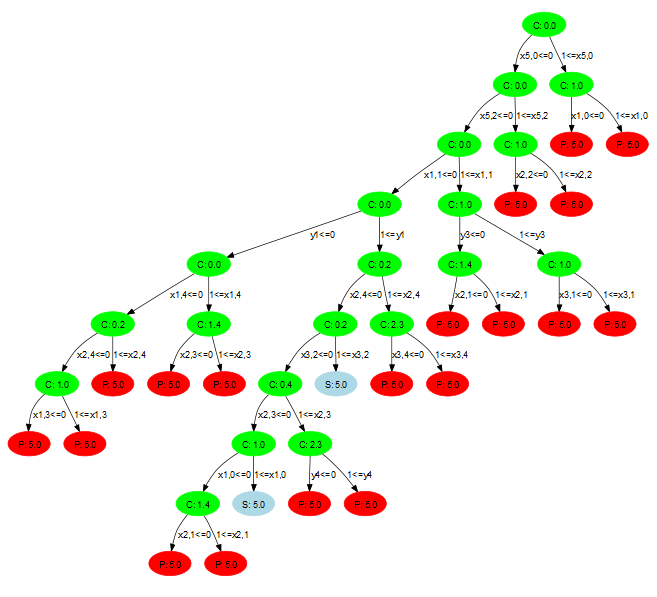
\includegraphics[bb=0 0 815 496,scale=0.50]{img/bpp_tree1.png}
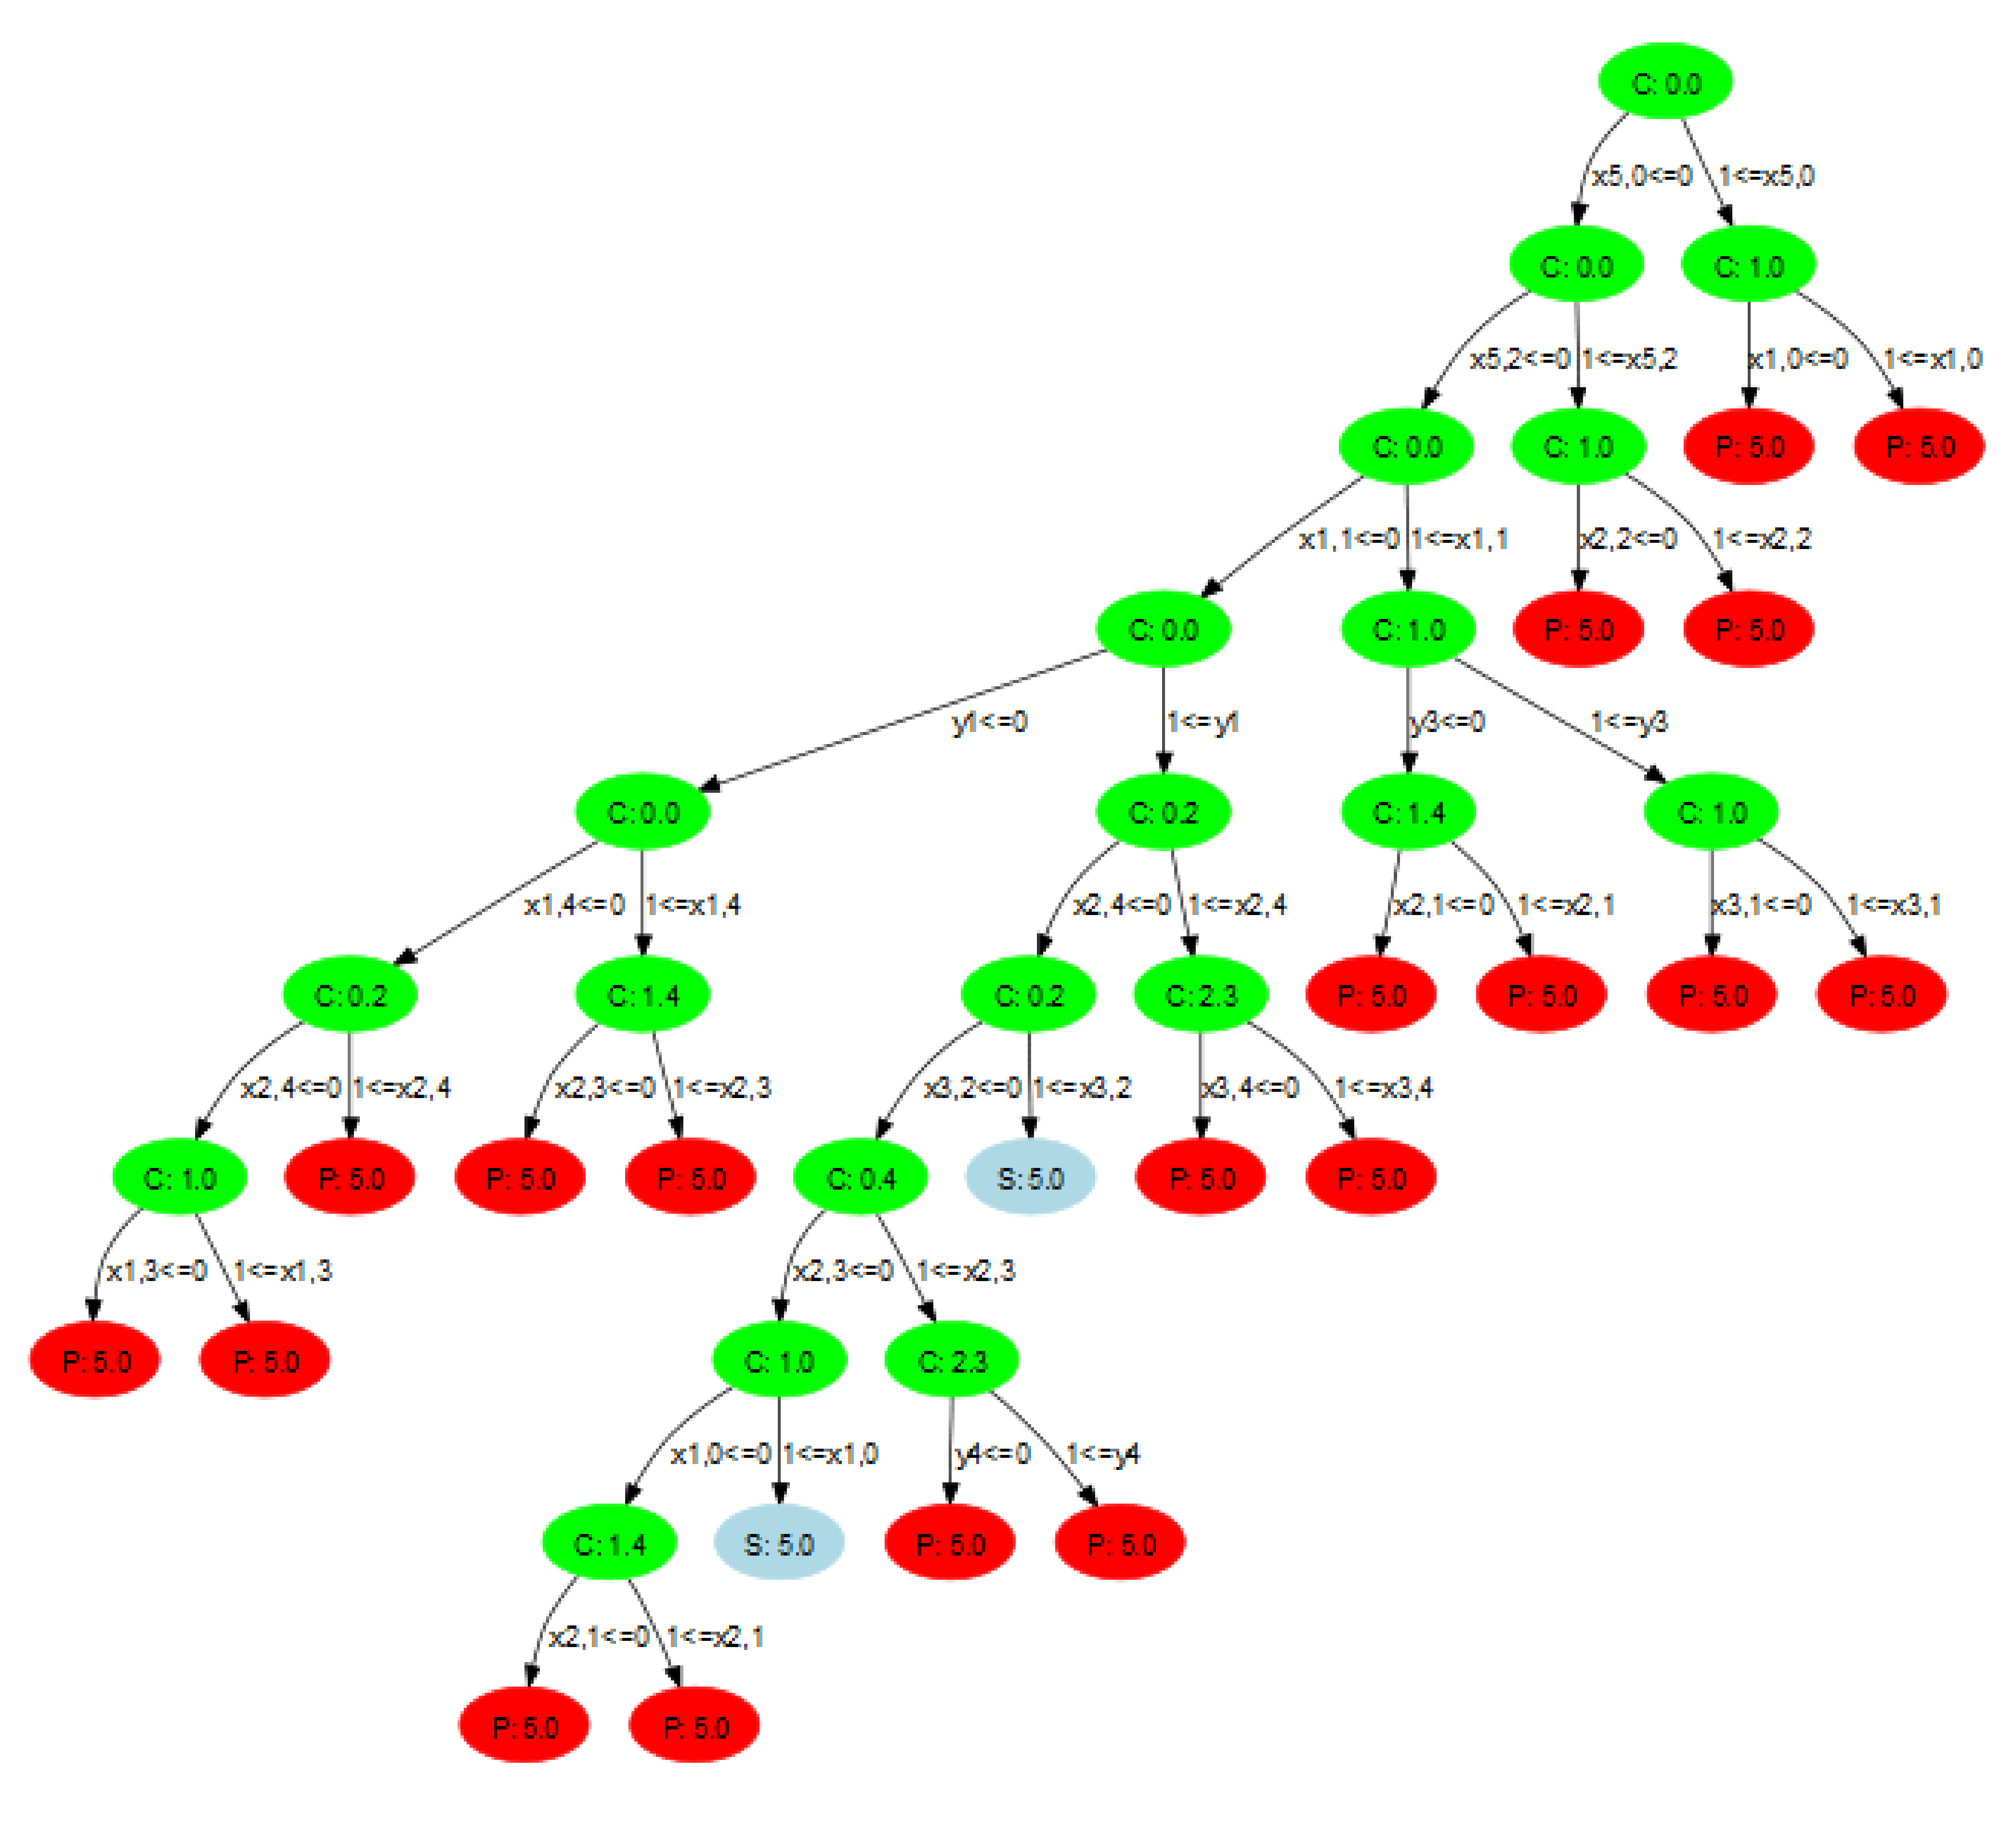
\includegraphics[scale=0.16]{img/bpp_tree1.eps}
\end{center}
\caption{Branch-and-bound tree for bin packing problem instance.} \label{fig:bpp_tree1}
\end{figure}

\newpage
Note that \ac{DIP} uses cuts from the \ac{CGL} \cite{coin_or} by default. We can turn \ac{CGL} cuts off by setting the {\tt CutCGL} flag in the \lstinline{dippyOpts} to \lstinline{'0'}.
\lstinputlisting[firstnumber=134,linerange={134-135,142-143}]{../../examples/Dippy/bpp/bin_pack_func.py}
The size of the branch-and-bound tree increases significantly  as shown in \figref{fig:bpp_tree4}.
\begin{figure}[htp]
\begin{center}
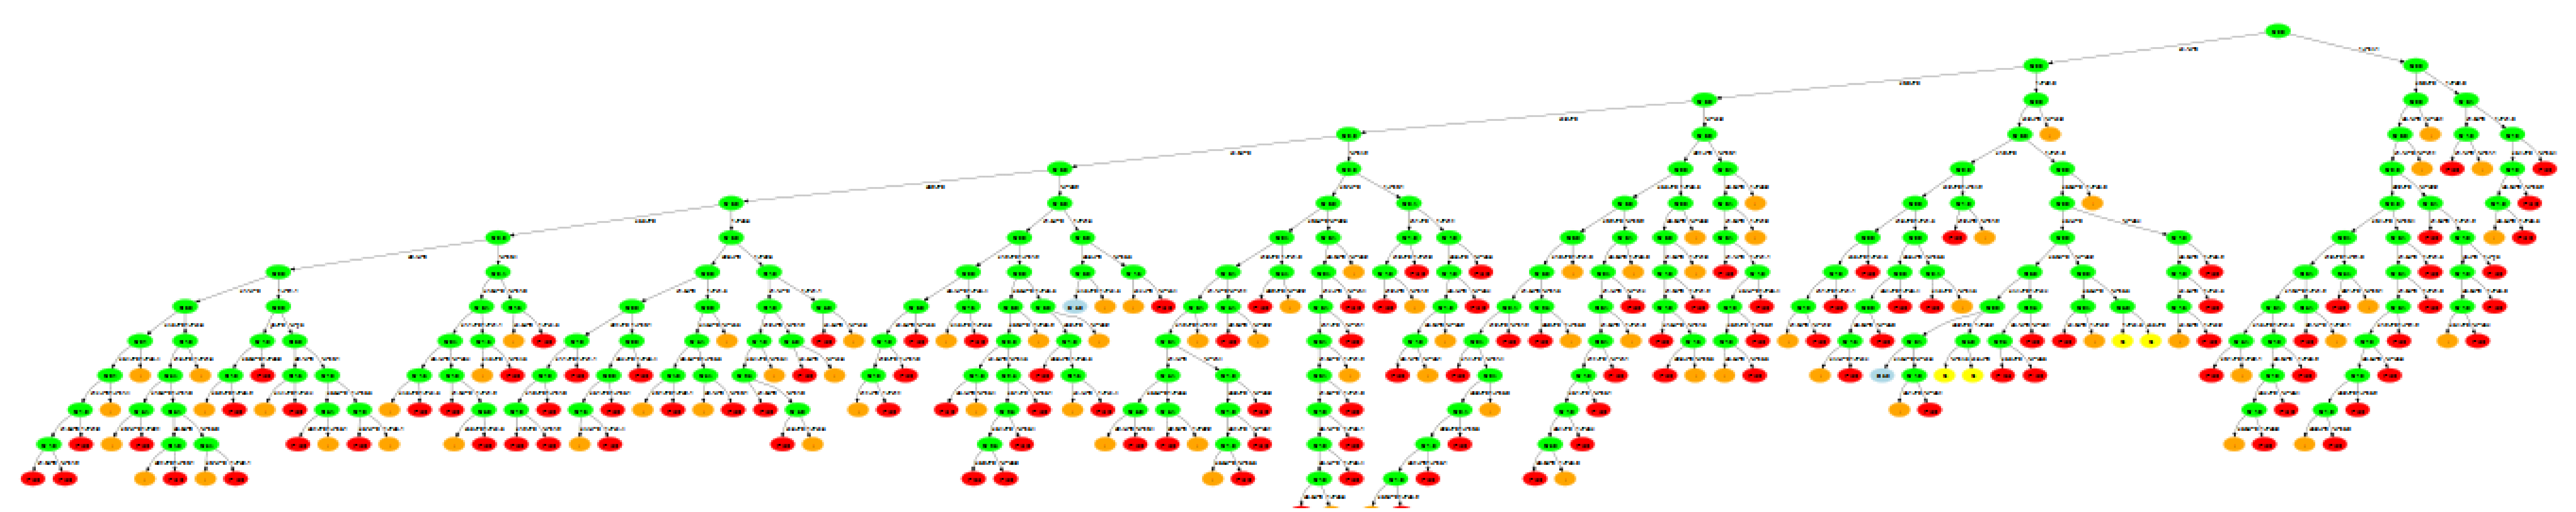
\includegraphics[scale=0.08]{img/bpp_tree4.eps}
\end{center}
\caption{Branch-and-bound tree for bin packing problem instance without \ac{CGL} cuts.} \label{fig:bpp_tree4}
\end{figure}



